\documentclass[11pt]{article}
\usepackage{amsmath, amssymb, array}
\pagestyle{plain}

\textwidth=6.5in
\hoffset-1in
\textheight=9in
\voffset-1in

\usepackage{enumitem}
\usepackage{pgfplots}
\usepackage{graphicx}
\usepackage{lipsum}
\usepackage{stfloats}
\usepackage{multicol}
\usepackage{minipage-marginpar}
\usepackage{tikz}
\setlength{\columnsep}{1cm}
\usepackage{pinlabel} % for pin labels on figure


\newcommand{\abs}[1]{\left| #1 \right|}


\begin{document}


\noindent MATH 1113   \quad\quad\quad\quad\quad Worksheet \quad\quad\quad\quad\quad\   Name \underline{\phantom{alphabetsoupismyveryveryfavorite}}\\ 
\noindent Final Exam Review\\




\noindent \textbf{Instructions:}  Work together in groups of  3 or 4 to complete the following problems.\\
\noindent Precalculus is the study of functions, how they can be expressed algebraically and graphically, their characteristics, and how they can be used to model concrete situations.\\

\noindent \underline{Types of Functions Studied}
\begin{enumerate}
\item linear
\item quadratic
\item exponential
\item logarithmic
\item trigonometric
\item polynomial (linear and quadratic functions are included in this category)
\end{enumerate}

\section{Linear Functions}
\begin{enumerate}



\item Circle the linear functions.

$$f(x)=3 \quad \quad g(x)=3x+5 \quad \quad h(x)=2x^3-x  \quad \quad k(x)=\cos(3x+7) \quad \quad j(x)=x$$

\item Let $f(x)$ be a linear function such that $\displaystyle f(-4)=1$ and the graph of $f(x)$ is parallel to the line $x+4y-3=0$. 
\begin{enumerate}
\item Determine $f(x)$ and write your final answer in \emph{slope-intercept} form. (Leave fractions in your answer, no decimals.)
\vfill
\newpage
\item Graph $f(x)$ and  $x+4y-3=0$ on the rectangular coordinate system below.\\
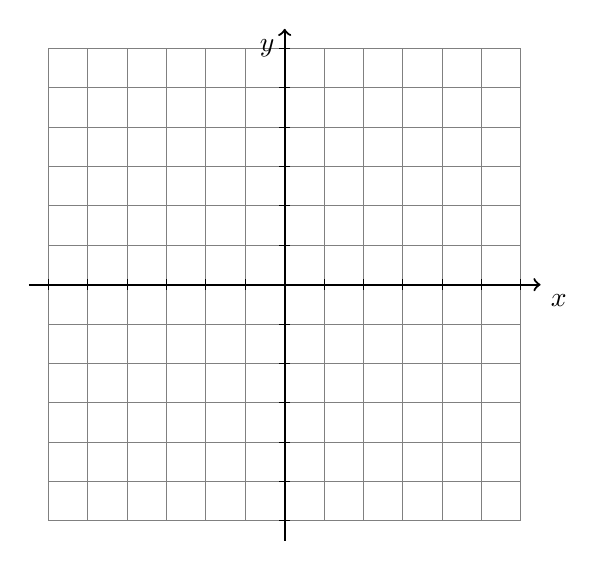
\begin{tikzpicture}[y=.5cm, x=0.5cm,font=\sffamily]
    %% ticks
    \draw[step = 1, gray] (-6,-6) grid (6,6);
    %% axis
    \draw[thick,->] (-6.5,0) -- coordinate (x axis mid) (6.5,0) node[anchor = north west] {$x$};
    \draw[thick,->] (0,-6.5) -- coordinate (y axis mid) (0,6.5) node[anchor = north east] {$y$};
    \foreach \y in {-6,-5,...,-1,1,2,...,6} {
      \draw (2pt, \y) -- (-2pt, \y);
    }
    \foreach \x in {-6,-5,...,-1,1,2,...,6} {
      \draw (\x,2pt) -- (\x,-2pt);
    }

  \end{tikzpicture}

\item Determine the domain and range of $f(x)$.\\[.3in]
\item Determine the inverse of $f(x)$.
\vfill
\end{enumerate}

\item A pediatrician records the age $x$ (in years) and average height $y$ (in inches) for girls between the ages of 2 and 10.

\begin{enumerate}
\item Use the points $(2,35)$ and $(6,46)$ to write a linear model for the data.
\vfill
\vfill
\item Interpret the meaning of the slope in context.
\vfill
\item Use the model to forecast the average height of 11 year old girls.
\vfill
\item If the height of a girl at age 11 is $90\%$ of her full-grown adult height, use the result of part $(c)$ to estimate the average height of adult women.  
\vfill

\end{enumerate}

\newpage
\section{Quadratic Functions}
\item Circle the quadratic functions.

$$f(x)=x \quad \quad g(x)=x^2-5 \quad \quad h(x)=3(x-4)^2+7  \quad \quad k(x)=3x^2+3x-1 \quad \quad j(x)=2^x$$


\item Write the standard (vertex) form of a parabola with vertex $(h,k)$.\\[.2in]

\item Given $f(x)=-2(x-1)^2+8$.

\begin{enumerate}

\item Determine whether the graph of the parabola opens upward or downward.\\[.2in]

\item Identify the vertex.\\[.2in]

\item Determine the $x$-intercept(s). (Remember that intercepts are points, not numbers.)
\vfill
\item Determine the $y$-intercept.
\vfill
\item Is it possible for a \textbf{function} to have more than one $y$-intercept?  Why or why not?\\[.2in]


\newpage
\item Determine the axis of symmetry of $f(x)$.\\[.2in]
\item Determine the maximum or minimum value of $f(x)$.
\vfill
\item Write the domain and range in interval notation.\\[.4in]
\item Graph $f(x)=-2(x-1)^2+8$.\\
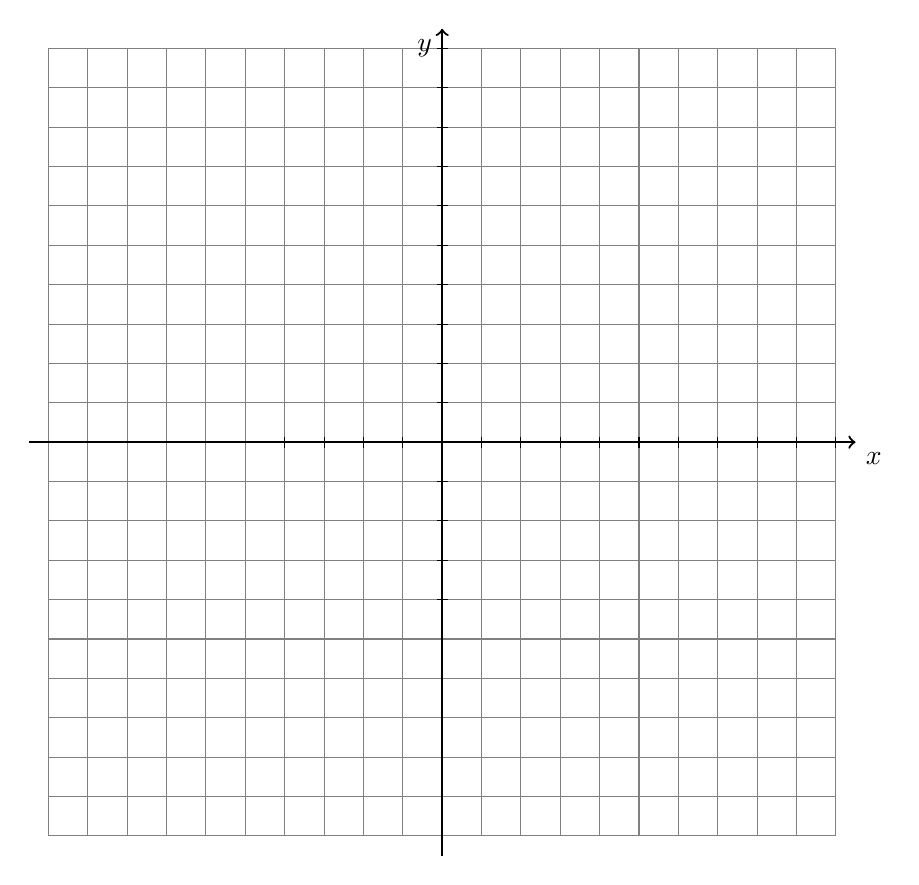
\begin{tikzpicture}[y=.5cm, x=0.5cm,font=\sffamily]
    %% ticks
    \draw[step = 1, gray] (-10,-10) grid (10,10);
    %% axis
    \draw[thick,->] (-10.5,0) -- coordinate (x axis mid) (10.5,0) node[anchor = north west] {$x$};
    \draw[thick,->] (0,-10.5) -- coordinate (y axis mid) (0,10.5) node[anchor = north east] {$y$};
    \foreach \y in {-4,-3,...,-1,1,2,...,10} {
      \draw (2pt, \y) -- (-2pt, \y);
    }
    \foreach \x in {-4,-3,...,-1,1,2,...,10} {
      \draw (\x,2pt) -- (\x,-2pt);
    }

  \end{tikzpicture}


\item Does the graph of $f(x)$ have an inverse?  If yes, find it.  If not, why?
\vfill
\end{enumerate}


\newpage


\item The monthly profit for a company that makes decorative picture frames depends on the price per frame.  The company determines that the profit is approximated by $f(p)=-80p^2+3440p-36,000$, where $p$ is the price per frame and $f(p)$ is the monthly profit based on that price.
\begin{enumerate}
\item Find the price that generates the maximum profit.
\vfill
\item Find the maximum profit.
\vfill
\item Find the price(s) that would enable the company to break even.
\vfill
\end{enumerate}

\item You have 50 cm of wire, and you have to use part of this wire to make a rectangle that's twice as long as it is wide, and the rest of the wire to make a square.  What should the dimensions of the shapes be if you want the total area to be as small as possible?  

\vfill
\vfill
\vfill

\newpage

\section{Exponential and Logarithmic Functions}
\item Circle the exponential functions.

$$f(x)=10^x \quad \quad g(x)=x^7 \quad \quad h(x)=3^{x-5}  \quad \quad k(x)=(x-5)^3 \quad \quad j(x)=e^x$$





\item Graph the functions and include their asymptotes and determine the domain and range of the functions.
\begin{multicols}{3}
\begin{enumerate}
\item $f(x)=2^x$
\columnbreak
\item $\displaystyle f(x)=\frac{1}{2}^x$
\columnbreak
\item $\displaystyle f(x)=2^{x-3}-5$
\end{enumerate}
\end{multicols}
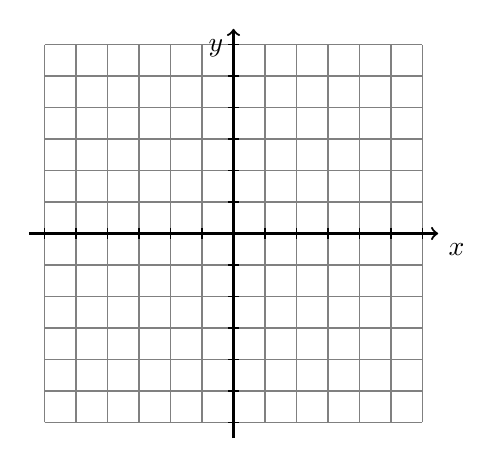
\begin{tikzpicture}[y=.4cm, x=0.4cm,font=\sffamily]
    %% ticks
    \draw[step = 1, gray] (-6,-6) grid (6,6);
    %% axis
    \draw[thick,->] (-6.5,0) -- coordinate (x axis mid) (6.5,0) node[anchor = north west] {$x$};
    \draw[thick,->] (0,-6.5) -- coordinate (y axis mid) (0,6.5) node[anchor = north east] {$y$};
    \foreach \y in {-6,-5,...,-1,1,2,...,6} {
      \draw (2pt, \y) -- (-2pt, \y);
    }
    \foreach \x in {-6,-5,...,-1,1,2,...,6} {
      \draw (\x,2pt) -- (\x,-2pt);
    }

  \end{tikzpicture}
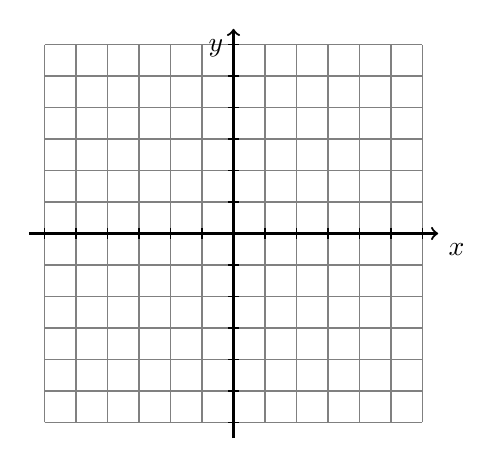
\begin{tikzpicture}[y=.4cm, x=0.4cm,font=\sffamily]
    %% ticks
    \draw[step = 1, gray] (-6,-6) grid (6,6);
    %% axis
    \draw[thick,->] (-6.5,0) -- coordinate (x axis mid) (6.5,0) node[anchor = north west] {$x$};
    \draw[thick,->] (0,-6.5) -- coordinate (y axis mid) (0,6.5) node[anchor = north east] {$y$};
    \foreach \y in {-6,-5,...,-1,1,2,...,6} {
      \draw (2pt, \y) -- (-2pt, \y);
    }
    \foreach \x in {-6,-5,...,-1,1,2,...,6} {
      \draw (\x,2pt) -- (\x,-2pt);
    }

  \end{tikzpicture}
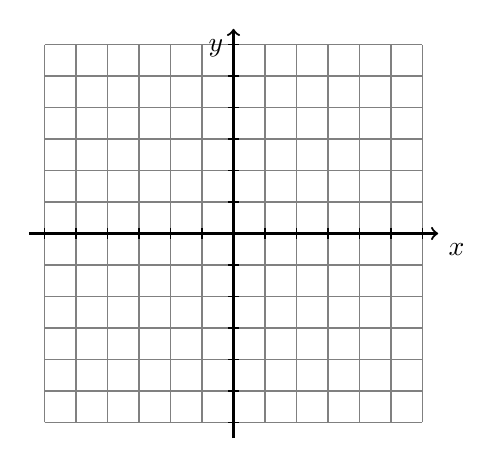
\begin{tikzpicture}[y=.4cm, x=0.4cm,font=\sffamily]
    %% ticks
    \draw[step = 1, gray] (-6,-6) grid (6,6);
    %% axis
    \draw[thick,->] (-6.5,0) -- coordinate (x axis mid) (6.5,0) node[anchor = north west] {$x$};
    \draw[thick,->] (0,-6.5) -- coordinate (y axis mid) (0,6.5) node[anchor = north east] {$y$};
    \foreach \y in {-6,-5,...,-1,1,2,...,6} {
      \draw (2pt, \y) -- (-2pt, \y);
    }
    \foreach \x in {-6,-5,...,-1,1,2,...,6} {
      \draw (\x,2pt) -- (\x,-2pt);
    }

  \end{tikzpicture}

\vfill
\item Graph the functions and include their asymptotes and determine the domain and range of the functions.
\begin{multicols}{3}
\begin{enumerate}
\item $f(x)=\log_2(x)$
\columnbreak
\item $\displaystyle f(x)=\log_{\frac{1}{2}}(x)$
\columnbreak
\item $\displaystyle f(x)=\log_2(x+5)+3$
\end{enumerate}
\end{multicols}

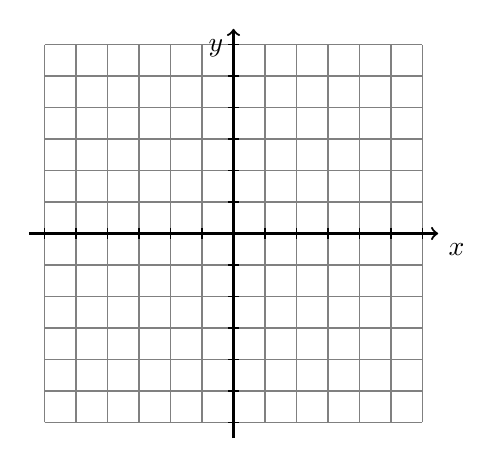
\begin{tikzpicture}[y=.4cm, x=0.4cm,font=\sffamily]
    %% ticks
    \draw[step = 1, gray] (-6,-6) grid (6,6);
    %% axis
    \draw[thick,->] (-6.5,0) -- coordinate (x axis mid) (6.5,0) node[anchor = north west] {$x$};
    \draw[thick,->] (0,-6.5) -- coordinate (y axis mid) (0,6.5) node[anchor = north east] {$y$};
    \foreach \y in {-6,-5,...,-1,1,2,...,6} {
      \draw (2pt, \y) -- (-2pt, \y);
    }
    \foreach \x in {-6,-5,...,-1,1,2,...,6} {
      \draw (\x,2pt) -- (\x,-2pt);
    }

  \end{tikzpicture}
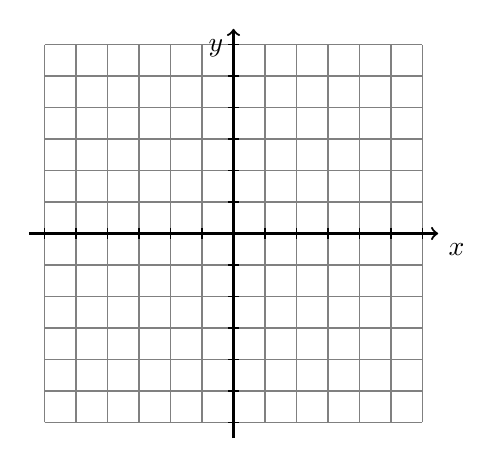
\begin{tikzpicture}[y=.4cm, x=0.4cm,font=\sffamily]
    %% ticks
    \draw[step = 1, gray] (-6,-6) grid (6,6);
    %% axis
    \draw[thick,->] (-6.5,0) -- coordinate (x axis mid) (6.5,0) node[anchor = north west] {$x$};
    \draw[thick,->] (0,-6.5) -- coordinate (y axis mid) (0,6.5) node[anchor = north east] {$y$};
    \foreach \y in {-6,-5,...,-1,1,2,...,6} {
      \draw (2pt, \y) -- (-2pt, \y);
    }
    \foreach \x in {-6,-5,...,-1,1,2,...,6} {
      \draw (\x,2pt) -- (\x,-2pt);
    }

  \end{tikzpicture}
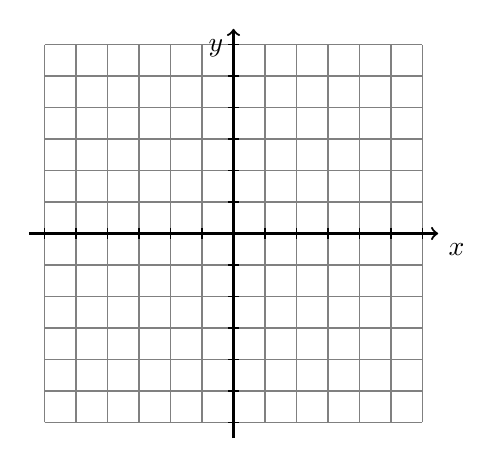
\begin{tikzpicture}[y=.4cm, x=0.4cm,font=\sffamily]
    %% ticks
    \draw[step = 1, gray] (-6,-6) grid (6,6);
    %% axis
    \draw[thick,->] (-6.5,0) -- coordinate (x axis mid) (6.5,0) node[anchor = north west] {$x$};
    \draw[thick,->] (0,-6.5) -- coordinate (y axis mid) (0,6.5) node[anchor = north east] {$y$};
    \foreach \y in {-6,-5,...,-1,1,2,...,6} {
      \draw (2pt, \y) -- (-2pt, \y);
    }
    \foreach \x in {-6,-5,...,-1,1,2,...,6} {
      \draw (\x,2pt) -- (\x,-2pt);
    }

  \end{tikzpicture}

\vfill


\newpage

\item Determine the inverse of the following functions.  (Hint:  you will need to rewrite in logarithmic or exponential form after switching $x$ and $y$.)  Then determine the domain and range of the function and its inverse.
\begin{enumerate}
\item $f(x)=\log_3(x+5)-7$
\begin{flushright}
Domain of $f(x)$:  \quad \quad \quad\quad\quad\quad Range of $f(x)$:\quad\quad\quad\quad \vfill
Domain of $f^{-1}(x)$:   \quad \quad\quad\quad\quad Range of $f^{-1}(x)$:\quad\quad\quad\quad
\end{flushright}
\vfill
\item $f(x)=5\ln(3x+4)$
\begin{flushright}
Domain of $f(x)$:  \quad \quad \quad\quad\quad\quad Range of $f(x)$:\quad\quad\quad\quad \vfill
Domain of $f^{-1}(x)$:   \quad \quad\quad\quad\quad Range of $f^{-1}(x)$:\quad\quad\quad\quad
\end{flushright}

\vfill 
\item $f(x)=7e^{2x+4}-3$
\begin{flushright}
Domain of $f(x)$:  \quad \quad \quad\quad\quad\quad Range of $f(x)$:\quad\quad\quad\quad \vfill 
Domain of $f^{-1}(x)$:   \quad \quad\quad\quad\quad Range of $f^{-1}(x)$:\quad\quad\quad\quad
\end{flushright}
\end{enumerate}

\newpage

\item $\$20,000$ is invested at $3.5\%$ interest compounded monthly.  How long will it take for the investment to double?

\vfill

\item On January 1, 2000, the population of Texas was approximately 21 million.  On January 1, 2010, the population was 25.2 million.

\begin{enumerate}
\item Write a function of the form $P(t)=P_0e^{kt}$ to represent the population $P(t)$ of Texas $t$ years after January 1, 2000.
\vfill 
\item Use the function in part $(a)$ to predict the population on January 1, 2020.
\vfill
\item Determine the year during which the population of Texas will reach 40 million if this trend continues.
\vfill
\end{enumerate}
\newpage


\section{Trigonometric Functions}



\item Graph $\displaystyle f(x)=2\cos(x+\frac{\pi}{2})-1$ and determine the domain and range.

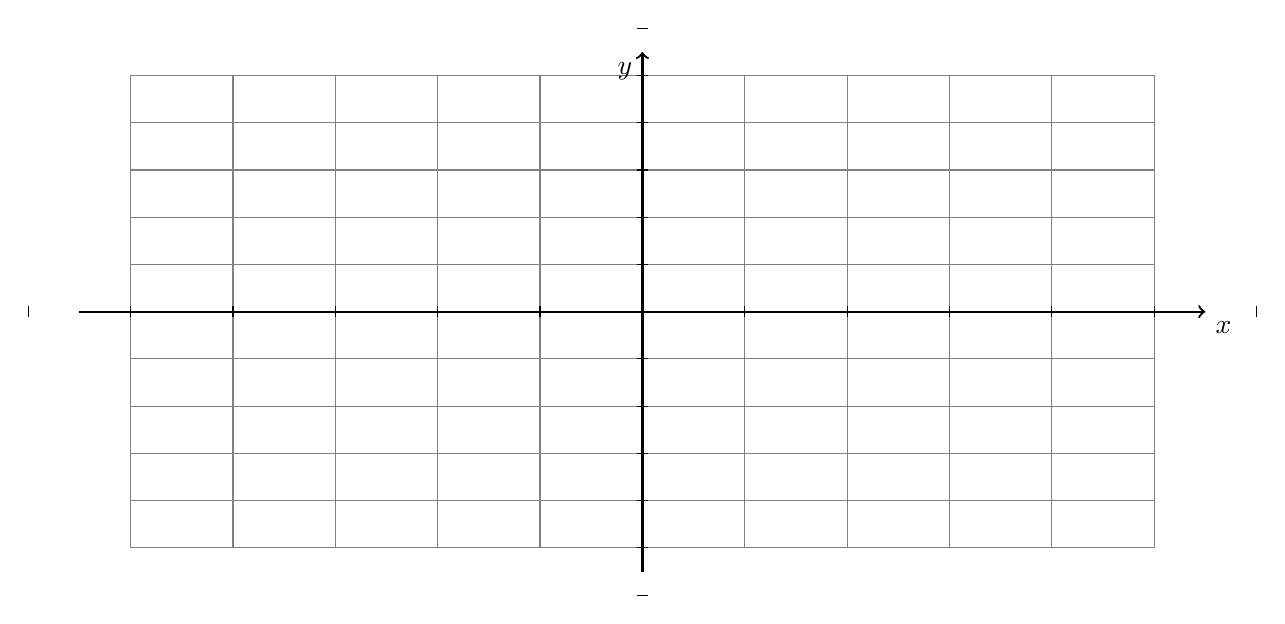
\begin{tikzpicture}[y=.6cm, x=1.3cm,font=\sffamily]
    %% ticks
    \draw[step = 1, gray] (-5,-5) grid (5,5);
    %% axis
    \draw[thick,->] (-5.5,0) -- coordinate (x axis mid) (5.5,0) node[anchor = north west] {$x$};
    \draw[thick,->] (0,-5.5) -- coordinate (y axis mid) (0,5.5) node[anchor = north east] {$y$};
    \foreach \y in {-6,-5,...,-1,1,2,...,6} {
      \draw (2pt, \y) -- (-2pt, \y);
    }
    \foreach \x in {-6,-5,...,-1,1,2,...,6} {
      \draw (\x,2pt) -- (\x,-2pt);
    }

  \end{tikzpicture}

\vfill
\item Graph $f(x)=-\sin(x+\pi)+2$ and determine the domain and range.

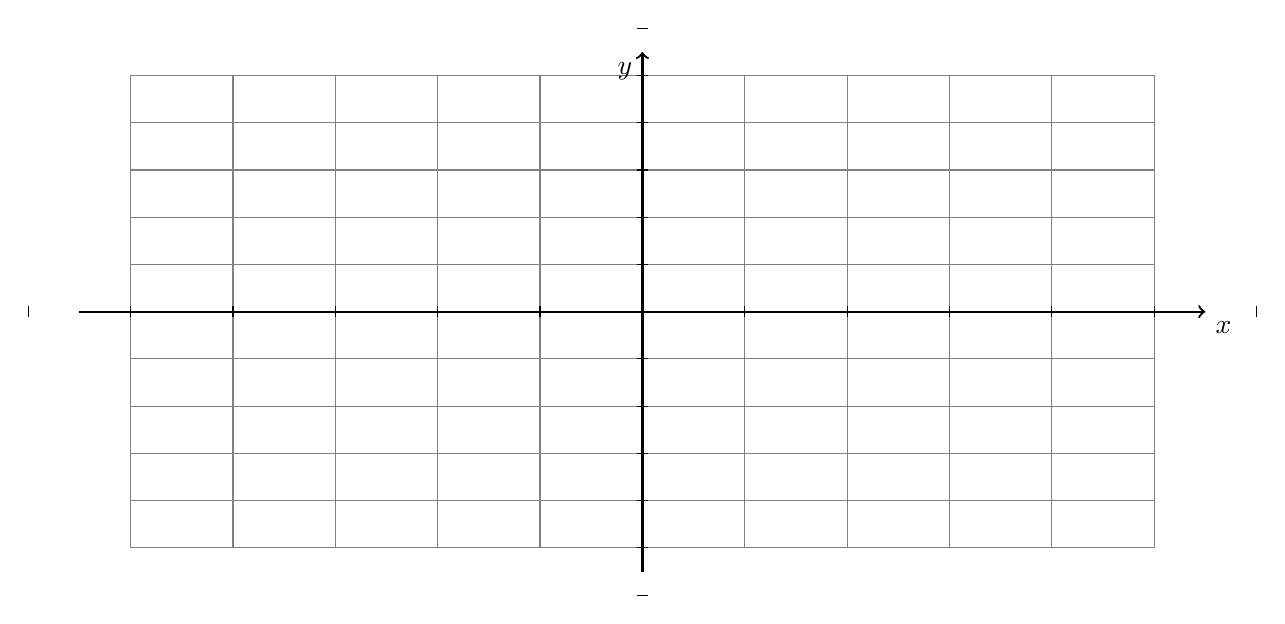
\begin{tikzpicture}[y=.6cm, x=1.3cm,font=\sffamily]
    %% ticks
    \draw[step = 1, gray] (-5,-5) grid (5,5);
    %% axis
    \draw[thick,->] (-5.5,0) -- coordinate (x axis mid) (5.5,0) node[anchor = north west] {$x$};
    \draw[thick,->] (0,-5.5) -- coordinate (y axis mid) (0,5.5) node[anchor = north east] {$y$};
    \foreach \y in {-6,-5,...,-1,1,2,...,6} {
      \draw (2pt, \y) -- (-2pt, \y);
    }
    \foreach \x in {-6,-5,...,-1,1,2,...,6} {
      \draw (\x,2pt) -- (\x,-2pt);
    }

  \end{tikzpicture}



\vfill



\newpage

\section{Polynomial Functions}

\item Sketch the graph of $f(x)=\frac{1}{10}(x-4)^2(2x+5)^3$.\\

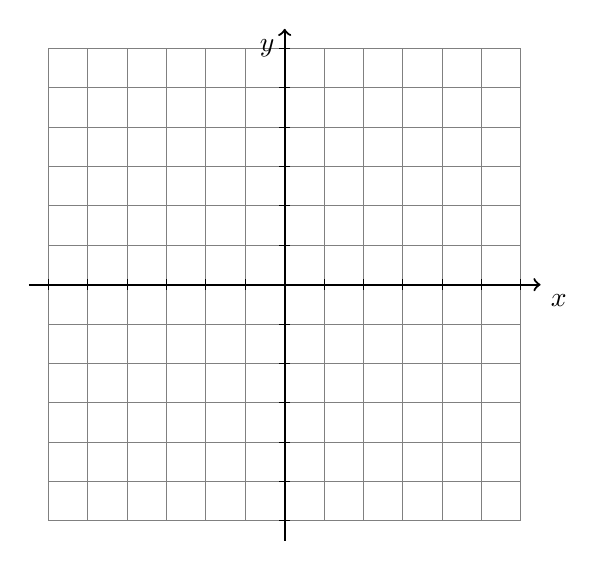
\begin{tikzpicture}[y=.5cm, x=0.5cm,font=\sffamily]
    %% ticks
    \draw[step = 1, gray] (-6,-6) grid (6,6);
    %% axis
    \draw[thick,->] (-6.5,0) -- coordinate (x axis mid) (6.5,0) node[anchor = north west] {$x$};
    \draw[thick,->] (0,-6.5) -- coordinate (y axis mid) (0,6.5) node[anchor = north east] {$y$};
    \foreach \y in {-6,-5,...,-1,1,2,...,6} {
      \draw (2pt, \y) -- (-2pt, \y);
    }
    \foreach \x in {-6,-5,...,-1,1,2,...,6} {
      \draw (\x,2pt) -- (\x,-2pt);
    }

  \end{tikzpicture}



\end{enumerate}

\end{document}